\documentclass[11pt]{article}
\usepackage[utf8]{inputenc}
\usepackage{amsmath,amssymb}
\usepackage{graphicx}
\usepackage{booktabs}
\usepackage{authblk}
\usepackage[margin=1in]{geometry}
\usepackage[hidelinks]{hyperref}
\usepackage{xurl}
\usepackage{setspace}
\usepackage{tikz}
\usepackage{pgfplots}
\pgfplotsset{compat=1.17}
\usetikzlibrary{arrows.meta,positioning,calc}

\title{Unified Coulomb Theory for Atom and Nuclear Physics}
\author[1]{Claes Johnson}
\affil[1]{KTH Royal Institute of Technology, SE-100 44 Stockholm, Sweden \\
\texttt{claesjohnson@gmail.com}}
\date{\today \\[0.4em]
\small\textit{Mathematical formulation and physical argument by the author; numerical} \\
\small\textit{implementation developed with AI assistance (Claude, Anthropic).}}

\begin{document}
\maketitle

\begin{abstract}
Atomic and nuclear physics are conventionally built on two different foundations: the atom on the
long-range Coulomb attraction between nuclei and electrons, the nucleus on a short-range strong force
between nucleons. We argue that a \emph{single} theory --- opposite-sign charge clouds interacting by
Coulomb forces alone, on non-overlapping spatial domains that meet at free boundaries, minimising the
electrostatic energy (\textbf{RealQM}) --- describes both, and that the atom and the nucleus are
related by \textbf{one operation: the swap electron $\leftrightarrow$ proton}. Because the two carry
opposite charge, the swap reverses every charge (charge conjugation); because they play opposite
structural roles, it simultaneously exchanges the compact confining \emph{kernel} with the mobile
\emph{valence} cloud. Because the kinetic energy takes the \emph{same form} for both species --- the mass of the charges
does not enter --- this swap is an \emph{exact symmetry} of the model, not an approximate analogy.
Under it the ladder of ordinary matter --- \emph{atom $\to$ molecule
$\to$ solid} --- maps term by term onto \emph{alpha $\to$ alpha-cluster $\to$ nuclear matter}. Closed
electron shells (the noble gases) correspond to closed proton shells (the $\alpha$-particle and the
$\alpha$-conjugate ``magic'' nuclei); covalent bonds by shared electrons correspond to nuclear bonds
by shared protons (nuclear molecules / $\alpha$-cluster states); the saturation of condensed matter
corresponds to nuclear saturation. Built from a single repeating unit, a $(2e^- + 4p)$ $\alpha$, the
computed $\alpha$-conjugate binding-energy ladder tracks experiment to $\sim\!107\%$ with
near-constant binding per nucleon --- from Coulomb forces and a single energy scale, with no strong or
weak force and no fitted parameters. Crucially the \emph{mass of the charges does not enter}: the
kinetic energy takes the same form for electrons and protons alike, which is precisely what makes the
swap an exact symmetry of the model rather than an approximate analogy. A single overall energy scale
is all that is calibrated, on the deuteron. A closer reading of the two scales suggests that it is
\emph{size}, not mass, that is the electromagnetic variable: the electron takes the proton's
(femtometre) size in the nucleus and an {\aa}ngstr\"om size $10^5$ times larger in the atom, at fixed
charge, the difference registered entirely in the kinetic energy. Mass enters the Coulomb energetics
only as an overall scale, not as a coupling in the Coulomb law, and on this reading belongs, with
gravitation, to a sector separate from electromagnetism. We give the correspondence, its quantitative
test, this size-not-mass reading, and the one genuine open
problem --- the free-boundary self-determination of geometry.

\medskip
\noindent\textbf{Keywords:} unified Coulomb model; RealQM; atomic structure; nuclear structure;
charge conjugation; electron--proton swap; $\alpha$ clustering; magic numbers; nuclear saturation;
size versus mass; mass and gravitation; free-boundary problems.
\end{abstract}

\setstretch{1.12}

\section{Introduction}

The Standard Model assigns atomic and nuclear binding to different interactions. Electrons bind to
nuclei, and atoms bind into molecules and solids, through the electromagnetic (Coulomb) force.
Nucleons bind into nuclei through the residual strong force, a short-range effective interaction
descended from quantum chromodynamics, while $\beta$-decay and the neutron's instability are governed
by the weak force. On this view the atom and the nucleus are structurally unrelated: they merely
happen to be concentric.

This paper advances the opposite thesis. We claim that a single physical model --- charge clouds of
both signs interacting by the Coulomb force alone --- reproduces the essential structure of
\emph{both} the atom and the nucleus, and that the two are not merely analogous but are
\emph{images of one another under a single operation}: the interchange of electron and proton. The
proton and the electron are the two stable unit charges of nature; swapping them, together with the
structural roles they play, carries every rung of atomic structure into a corresponding rung of
nuclear structure.

The model is \textbf{RealQM}~\cite{Johnson-RealQM,Johnson-Book}, a deterministic real-space
reformulation of quantum mechanics in which the state is a charge density partitioned into
one-particle components on non-overlapping domains separated by free boundaries, and the ground state
minimises the classical Coulomb energy. RealQM reproduces the periodic table and molecular binding
from electrostatics~\cite{Johnson-Atoms}; applied to nucleons it yields nuclear binding without a
strong force~\cite{Johnson-RealNucleus}. Here we do not re-derive those computations but organise them
into a single statement: atomic and nuclear matter are the two faces of one Coulomb theory, exchanged
by $e^-\!\leftrightarrow p$.

We are explicit about what is and is not claimed. We do not claim to reproduce quantum chromodynamics,
scattering phase shifts, or the fine detail of the nuclear force. We claim that the \emph{gross
structure} of nuclei --- the special stability of the $\alpha$-particle, the $\alpha$-conjugate and
magic nuclei, $\alpha$-clustering, the weak binding of $^8$Be, saturation and near-constant binding
per nucleon --- follows, quantitatively at the $\sim\!10\%$ level, from Coulomb forces alone once the
electron--proton swap is taken seriously, and that this same structure is the charge conjugate of
ordinary chemistry.

\section{The RealQM framework}

In RealQM the total charge distribution is a sum
\begin{equation}
\Psi(x) \;=\; \sum_{i=1}^{N}\psi_i(x),
\end{equation}
of $N$ one-particle real-valued components $\psi_i$, each carrying unit charge $q_i=\pm 1$ and
supported on its own spatial domain $\Omega_i$. The domains are \emph{non-overlapping}, tiling the
region occupied by the system,
\begin{equation}
\Omega_i \cap \Omega_j = \emptyset \quad (i\neq j), \qquad \bigcup_i \Omega_i = \Omega,
\end{equation}
and neighbouring domains meet at internal interfaces $\Gamma_{ij}=\partial\Omega_i\cap\partial\Omega_j$
whose location is \emph{not prescribed} but is part of the unknown: a \emph{free boundary}. The state
minimises the energy
\begin{equation}
E[\{\psi_i\},\{\Omega_i\}] \;=\;
\sum_i \frac{1}{2}\!\int_{\Omega_i}\!|\nabla\psi_i|^2\,dx
\;+\; \tfrac{1}{2}\!\iint \frac{\rho(x)\,\rho(y)}{|x-y|}\,dx\,dy,
\qquad \rho=\sum_i q_i\,\psi_i^2,
\label{eq:energy}
\end{equation}
subject to normalisation $\int_{\Omega_i}\psi_i^2\,dx=1$ of each component. The first term is the
quantum kinetic (zero-point) energy, written with the \emph{same form for every component} --- the same
operator $|\nabla\psi_i|^2$ for electrons and protons alike, so that the mass of the charges does not
enter as a parameter; the second is the classical electrostatic self-energy of the total charge density
$\rho$, and is the \emph{only} interaction in the model. There is no exchange term, no correlation functional, and no
many-body wavefunction on configuration space --- only densities in ordinary three-space and the free
boundaries between them.

Minimisation over the component shapes gives, on each domain, a one-particle Schr\"odinger-type
equation in the self-consistent Coulomb potential $\phi=\sum_j q_j\,\psi_j^2 * |x|^{-1}$; minimisation
over the free boundaries gives a \emph{continuity condition} on the charge density across each
interface (a Bernoulli-type free-boundary condition balancing the densities of the two adjacent
components). Physically: each charge cloud is confined by the Coulomb field of its neighbours, and the
interfaces float to where the confining pressures balance. This single principle --- \emph{mutual
Coulomb confinement of charge clouds with floating interfaces} --- is all that follows below.

A physical setting is specified by the \emph{signs and multiplicities} of the charges together with a
single overall energy scale. The \emph{masses do not enter}: the kinetic term has the same form for
every cloud, so an electron cloud and a proton cloud are distinguished only by the sign of their
charge. This is what makes the swap $e^-\!\leftrightarrow p$ an exact symmetry of the functional
(Sec.~\ref{sec:mass}). Everything else is output.

\section{The electron--proton swap}

\begin{figure}[t]
\centering
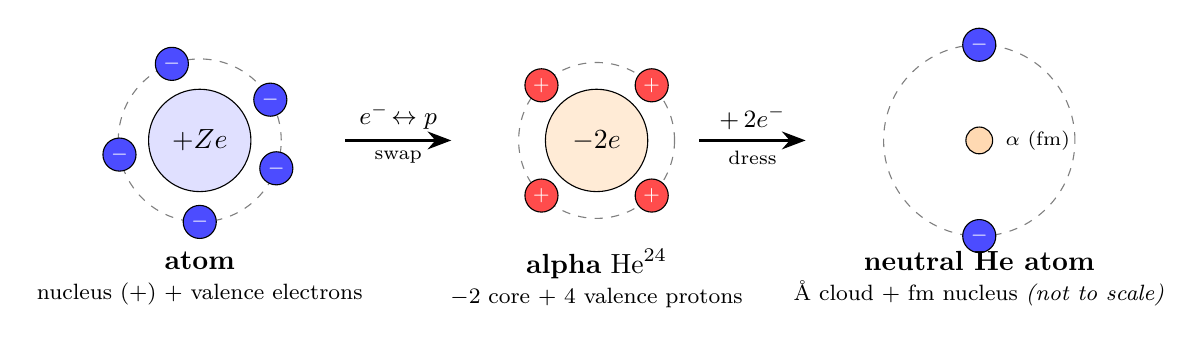
\begin{tikzpicture}[scale=0.9,
  kernelpos/.style={circle,draw,fill=blue!12,minimum size=13mm,inner sep=0pt},
  kerneln/.style={circle,draw,fill=orange!16,minimum size=13mm,inner sep=0pt},
  pdot/.style={circle,draw,fill=red!70,text=white,minimum size=4.2mm,inner sep=0pt,font=\scriptsize},
  edot/.style={circle,draw,fill=blue!70,text=white,minimum size=4.2mm,inner sep=0pt,font=\scriptsize},
  alphadot/.style={circle,draw,fill=orange!30,minimum size=3.4mm,inner sep=0pt}]

 % ---- atom ----
 \node[kernelpos] (K) at (0,0) {$+Ze$};
 \draw[dashed,gray] (0,0) circle (1.15);
 \foreach \a in {30,110,190,270,340} \node[edot] at (\a:1.15) {$-$};
 \node[align=center] at (0,-1.95) {\textbf{atom}\\[-1pt]\footnotesize nucleus (+) $+$ valence electrons};

 % ---- swap arrow ----
 \draw[-{Stealth[length=3mm]},very thick] (2.05,0) -- (3.55,0)
   node[midway,above,font=\small] {$e^-\!\leftrightarrow p$}
   node[midway,below,font=\scriptsize] {swap};

 % ---- alpha ----
 \node[kerneln] (C) at (5.6,0) {$-2e$};
 \draw[dashed,gray] (5.6,0) circle (1.1);
 \foreach \a in {45,135,225,315} \node[pdot] at ($(5.6,0)+(\a:1.1)$) {$+$};
 \node[align=center] at (5.6,-1.95) {\textbf{alpha} $\mathrm{He}^{24}$\\[-1pt]\footnotesize $-2$ core $+$ $4$ valence protons};

 % ---- dress with 2 outer electrons ----
 \draw[-{Stealth[length=3mm]},very thick] (7.05,0) -- (8.55,0)
   node[midway,above,font=\small] {$+\,2e^-$}
   node[midway,below,font=\scriptsize] {dress};

 % ---- neutral He atom: outer cloud (A) around tiny alpha (fm) ----
 \begin{scope}[shift={(11.0,0)}]
   \draw[dashed,gray] (0,0) circle (1.35);
   \node[edot] at (90:1.35) {$-$};
   \node[edot] at (270:1.35) {$-$};
   \node[alphadot] (a) at (0,0) {};
   \node[font=\scriptsize,right=1pt of a] {$\alpha$ (fm)};
 \end{scope}
 \node[align=center] at (11.0,-1.95) {\textbf{neutral He atom}\\[-1pt]\footnotesize \AA\ cloud $+$ fm nucleus \emph{(not to scale)}};
\end{tikzpicture}
\caption{The electron--proton swap, and the two scales in one atom. \emph{(Left)} An atom is a positive
nuclear kernel dressed by negative valence electrons; applying $e^-\!\leftrightarrow p$ turns it into
the $\alpha$-particle ($\mathrm{He}^{24}$) --- a negative $-2$ electron core dressed by four positive
valence protons --- reversing every charge and exchanging the roles of confining kernel and mobile
valence cloud. \emph{(Right)} The same $\alpha$ dressed by two outer electrons is a neutral helium
atom, which displays both scales at once: an {\aa}ngstr\"om-scale electron cloud around a
femtometre-scale nucleus (not to scale), cf.\ Eq.~\eqref{eq:He-two-scales}.}
\label{fig:swap}
\end{figure}

The proton and the electron are the two stable elementary charges. Consider the single operation
\begin{equation}
\boxed{\;e^-\;\longleftrightarrow\;p\;}
\end{equation}
that interchanges them everywhere in a structure. Because $q_{e}=-1$ and $q_{p}=+1$, the swap reverses
the sign of every charge --- it is charge conjugation at the level of the charge density. But it does
more: in ordinary matter the \emph{proton(s)} form the compact heavy kernel and the \emph{electrons}
form the light mobile valence cloud, so interchanging the two species also interchanges the
\emph{structural roles} of kernel and valence. The swap is therefore simultaneously
\begin{center}
(charge conjugation) $\;+\;$ (kernel $\leftrightarrow$ valence).
\end{center}

Read at the level of a single unit (Fig.~\ref{fig:swap}):
\[
\underbrace{\text{atom}}_{\text{nucleus}\,(+)\ \oplus\ \text{electrons}\,(-)}
\quad\xrightarrow{\;e^-\leftrightarrow p\;}\quad
\underbrace{\text{alpha}}_{\text{electron core}\,(-)\ \oplus\ \text{protons}\,(+)} .
\]
Read at the level of a bound assembly:
\[
\underbrace{\text{molecule}}_{\text{nuclei glued by shared }e^-}
\quad\xrightarrow{\;e^-\leftrightarrow p\;}\quad
\underbrace{\text{nucleus / nuclear matter}}_{\alpha\text{'s glued by shared }p} .
\]
The full correspondence is the ladder of Table~\ref{tab:correspondence}, obtained by applying the one
swap at each rung. In RealQM the neutron is not elementary but a bound proton--electron pair
$n=(p\,e^-)$~\cite{Johnson-RealNucleus}, so a nucleus $^{A}_{Z}X$ is simply $A$ protons and $A-Z$
electrons --- charge clouds of both signs, the very same objects as an atom, related to it by the
swap. The remainder of the paper substantiates each rung.

\begin{table}[t]
\centering
\renewcommand{\arraystretch}{1.25}
\begin{tabular}{ll}
\toprule
\textbf{Ordinary matter} & \textbf{Nucleus (after $e^-\!\leftrightarrow p$)}\\
\midrule
nucleus --- positive kernel                      & $-2$ electron core --- negative kernel\\
\textbf{atom} $=$ kernel $+$ valence electrons    & \textbf{alpha} $=$ $-2$ core $+$ valence protons\\
\textbf{molecule} $=$ atoms $+$ shared electrons  & \textbf{alpha cluster} $=$ alphas $+$ shared protons\\
solid / metal                                    & heavy nucleus / nuclear matter\\
\bottomrule
\end{tabular}
\caption{The charge-conjugate correspondence between atomic and nuclear matter, generated by the
single swap $e^-\!\leftrightarrow p$. The confining kernel is positive (the nucleus) in the atom and
negative (the $-2$ electron core) in the nucleus; the mobile valence species is the electron in one
regime and the proton in the other.}
\label{tab:correspondence}
\end{table}

\section{Kernel and valence: the atom and the alpha}

An \textbf{atom} is a compact positive kernel (the nucleus) surrounded by negative valence electrons
in shells. The kernel confines the electrons by Coulomb attraction; the electrons screen the kernel.
Shell closure at $2,10,18,\dots$ electrons defines the chemically inert \emph{noble gases}, whose
special stability is the organising fact of the periodic table~\cite{MayerJensen}.

Applying $e^-\!\leftrightarrow p$ produces the \textbf{alpha} ($^4$He nucleus): a compact negative
kernel --- two electrons forming a closed $-2$ core --- surrounded by four positive valence protons.
The core confines the protons by Coulomb attraction; the protons cage the core. This is a closed,
saturated shell, and the $\alpha$-particle is correspondingly the \emph{most tightly bound light
nucleus per nucleon} and chemically-nuclearly inert: the \textbf{nuclear noble gas}. Its four-proton
closure is the image of a filled electron shell, and the sequence of especially bound closed-shell
nuclei --- the $\alpha$-conjugate nuclei $^4$He, $^{12}$C, $^{16}$O, $^{20}$Ne, $^{24}$Mg, $\dots$,
and more generally the \emph{magic numbers}~\cite{MayerJensen,HaxelJensenSuess} --- is the nuclear
image of the noble-gas column. Both express the same rule, \emph{closed shell $=$ specially stable},
read in opposite charge under the swap.

\section{Bonding: the molecule and the alpha cluster}

A \textbf{molecule} forms when atoms share their valence \emph{electrons}: negative charge concentrates
in the seam between two positive kernels, attracted to both, and this shared electron density is the
covalent bond~\cite{Johnson-Atoms}. Closed-shell atoms (noble gases) share reluctantly and bond only
weakly (van der Waals); open-shell atoms bond strongly.

The swap turns this into the \textbf{alpha cluster}: a nucleus built of several $\alpha$'s that bond
by sharing their valence \emph{protons}. A proton in the seam between two $\alpha$'s is attracted to
\emph{both} negative $-2$ cores, and this shared positive charge is the bond. It must be the proton,
not the electron: between two negative kernels only positive charge is bonding, since an electron
placed there is repelled by both cores. And, exactly as in chemistry, the closed-shell $\alpha$ shares
reluctantly, so the inter-$\alpha$ bond is \emph{weak}:
\begin{itemize}\setlength{\itemsep}{2pt}
\item $^8$Be (two $\alpha$'s) is the barely-bound ``He$_2$ dimer'' of nuclei --- unbound by only
$\sim\!92$~keV, a resonance that promptly decays into two $\alpha$'s, precisely as a noble-gas dimer is
barely bound;
\item $^{12}$C and $^{16}$O are stable small ``molecules'' of three and four $\alpha$'s, the latter
with the tetrahedral symmetry of a well-coordinated cluster; the Hoyle state of
$^{12}$C~\cite{Hoyle,THSR} is a loose, gas-like three-$\alpha$ molecule.
\end{itemize}
This is exactly the object nuclear physics already names an \emph{$\alpha$-cluster state} or
\emph{nuclear molecule}, systematised in the Ikeda threshold diagram~\cite{Ikeda} and reviewed
extensively~\cite{FreerRPP,FreerRMP,vonOertzen}. What the swap contributes is its \emph{origin}: the
$\alpha$-cluster state is the charge conjugate of a chemical molecule, and its weakness is the
charge conjugate of noble-gas inertness --- both from Coulomb alone.

\section{Bulk: solids and nuclear matter; why clustering is forced}

Extended matter is the last rung. A \textbf{solid or metal} is a lattice of positive kernels held by a
shared sea of negative electrons; its binding is \emph{extensive} (energy $\propto$ number of atoms),
a saturation that follows from the screening of the long-range Coulomb interaction in a globally
neutral medium. Under the swap, \textbf{nuclear matter} --- a heavy nucleus --- is many $\alpha$ units
in a common medium of shared protons, binding extensively with near-constant binding per nucleon,
which is precisely nuclear \emph{saturation}~\cite{BetheWeizsacker}.

Saturation is not merely reproduced; it \emph{forces the cluster structure}. Consider concentrating
all the glue at a single centre --- a ``monolithic'' nucleus in which every proton shares one
long-range Coulomb well. The electrostatic energy of $Z$ mutually-attracted charges in a common well
grows as $Z^2$, so a monolithic nucleus \emph{over-binds}, its binding per nucleon rising without
bound. This is confirmed directly in RealQM: monolithic $^8$Be, $^{16}$O, $\dots$ over-bind with a
ratio to experiment scaling as $\sim\!Z^2$~\cite{Johnson-RealNucleus}. Real nuclear binding is
extensive ($\propto A$), and the only way to obtain extensivity from a long-range $1/r$ interaction is
to \emph{localise the glue into charge-neutral, $\alpha$-sized packets} --- i.e. to cluster.
$\alpha$-clustering is therefore not optional in this picture but \emph{required}: it is the mechanism
that converts long-range Coulomb attraction into an effectively short-range, saturating interaction,
the same role that screening plays in a metal. The swap thus explains not only \emph{that} nuclei
cluster but \emph{why} they must.

\section{Quantitative test: the alpha-conjugate ladder}

The correspondence is testable, not merely pictorial. Building each nucleus from the single repeating
unit --- a $(2e^- + 4p)$ $\alpha$, the electron pair inside and the proton quartet outside --- and
computing the RealQM ground-state energy~\eqref{eq:energy} with one energy scale fixed on the
deuteron, the $\alpha$-conjugate ladder reproduces the experimental binding energies to a uniform
$\sim\!107\%$ with near-constant binding per nucleon~\cite{Johnson-RealNucleus}.
Table~\ref{tab:ladder} lists the experimental values and Fig.~\ref{fig:bpa} shows the computed track
against them; the flat plateau near $8$~MeV per nucleon is nuclear saturation, emerging here from
electromagnetism and structure alone.

\begin{table}[h]
\centering
\renewcommand{\arraystretch}{1.15}
\begin{tabular}{lcccc}
\toprule
Nucleus & $\#\alpha$ & $B_{\exp}$ (MeV) & $B_{\exp}/A$ (MeV) & RealQM $B/A$ (Coulomb only)\\
\midrule
$^{4}$He   & 1 & 28.30  & 7.07 & $\approx 1.07\times$ exp\\
$^{12}$C   & 3 & 92.16  & 7.68 & $\approx 1.07\times$ exp\\
$^{16}$O   & 4 & 127.62 & 7.98 & $\approx 1.07\times$ exp\\
$^{20}$Ne  & 5 & 160.64 & 8.03 & $\approx 1.07\times$ exp\\
$^{24}$Mg  & 6 & 198.26 & 8.26 & $\approx 1.07\times$ exp\\
$^{28}$Si  & 7 & 236.54 & 8.45 & $\approx 1.07\times$ exp\\
$^{32}$S   & 8 & 271.78 & 8.49 & $\approx 1.07\times$ exp\\
$^{40}$Ca  &10 & 342.05 & 8.55 & $\approx 1.08\times$ exp\\
\bottomrule
\end{tabular}
\caption{The $\alpha$-conjugate ladder. Experimental binding energies $B_{\exp}$ and binding per
nucleon $B_{\exp}/A$ (evaluated data). The RealQM computation from Coulomb alone, one scale fixed on
the deuteron and no other parameter, tracks these uniformly at $\sim\!107\%$ with near-constant $B/A$;
per-nucleus computed values and the imposed-geometry protocol are given in the companion
work~\cite{Johnson-RealNucleus}.}
\label{tab:ladder}
\end{table}

\begin{figure}[h]
\centering
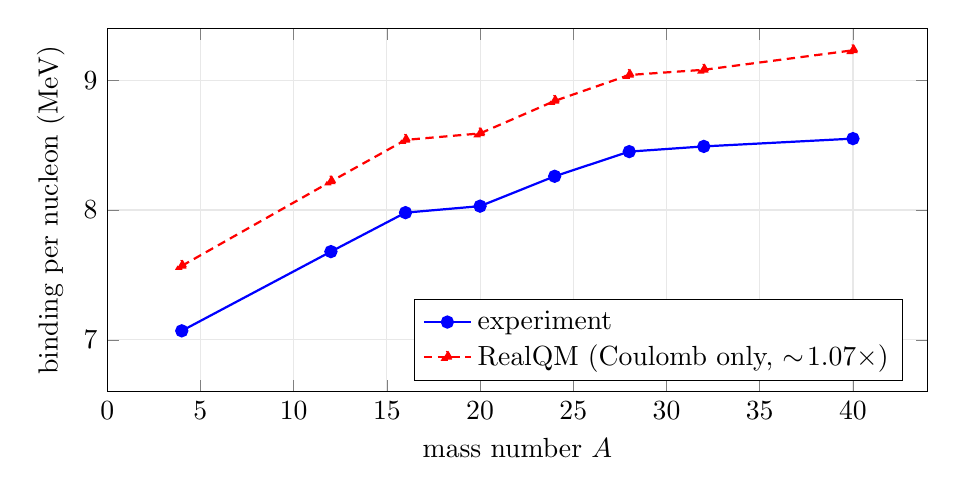
\begin{tikzpicture}
\begin{axis}[
  width=12cm,height=6.2cm,
  xlabel={mass number $A$}, ylabel={binding per nucleon (MeV)},
  xmin=0,xmax=44,ymin=6.6,ymax=9.4,
  grid=both, grid style={gray!18},
  legend pos=south east, legend cell align=left,
  every axis plot/.append style={thick},
]
% experimental B/A for alpha-conjugate nuclei
\addplot[mark=*,blue] coordinates {
 (4,7.07)(12,7.68)(16,7.98)(20,8.03)(24,8.26)(28,8.45)(32,8.49)(40,8.55)};
\addlegendentry{experiment}
% RealQM (Coulomb only), ~1.07 x exp
\addplot[mark=triangle*,red,densely dashed] coordinates {
 (4,7.57)(12,8.22)(16,8.54)(20,8.59)(24,8.84)(28,9.04)(32,9.08)(40,9.23)};
\addlegendentry{RealQM (Coulomb only, $\sim\!1.07\times$)}
\end{axis}
\end{tikzpicture}
\caption{Binding per nucleon along the $\alpha$-conjugate ladder: experiment (solid) and the RealQM
Coulomb-only computation (dashed, $\sim\!107\%$ of experiment), both showing the saturation plateau
and its slow rise toward the iron region. No strong force and no fitted parameter enters; the single
energy scale is fixed on the deuteron~\cite{Johnson-RealNucleus}.}
\label{fig:bpa}
\end{figure}

The benchmark deserves one clarification, because the comparison is a parameter-free prediction placed
against a nearly model-free measurement. What is \emph{directly measured} for a nucleus are the three
masses --- proton, neutron, nucleus --- weighed to high precision. The binding energy is then
\emph{inferred} as the mass deficit via $E=mc^2$, relative to the chosen decomposition into $Z$
protons and $N$ neutrons. No nuclear model enters this inference. RealQM, on the other side, computes a
binding energy from Coulomb forces with nothing fitted. The agreement in Fig.~\ref{fig:bpa} is thus
between a Coulomb computation and a mass-deficit measurement, on the single scale set by the deuteron.

\section{Computing the geometry: the metastable alpha}

The bindings above are computed at \emph{imposed} geometry: radii chosen at each size, only the clouds
relaxed. The stronger test releases the nucleons and lets the free boundary and the force balance fix
the geometry as output. Carried out for the $\alpha$~\cite{Johnson-RealNucleus}, the result is precise
and instructive:
\begin{itemize}\setlength{\itemsep}{2pt}
\item The isolated $\alpha$ does \emph{not} sit at a strict compact minimum. Glued only from the
inside, its four mutually-repelling protons slowly spread, and the energy \emph{falls} as they do --- so
the drift is physical, not numerical.
\item But the compact form is long-lived \emph{metastable}: with a gentler boundary evolution the
energy read at the compact point ($E\approx-32$ in model units) matches the imposed value ($-31.8$)
before the drift sets in. The compact $\alpha$ is thus computable as a metastable state.
\item Four \emph{separated} $\alpha$'s (each net $+2$) repel and disperse, consistent with the model
disfavouring widely-separated droplets.
\end{itemize}
This closes the loop with the swap. The missing ingredient for the isolated $\alpha$ is \emph{outer
confinement}, which only neighbours can supply --- exactly what a cluster provides. In an
$\alpha$-cluster the surrounding units hold each $\alpha$ fixed at the metastable compact size it would
otherwise leave: a decaying plateau for one $\alpha$ is a genuine minimum for the cluster. The isolated
$\alpha$'s near-self-binding and the strong $\alpha$-clustering of nuclei are therefore \emph{one
fact}, the nuclear image of chemical bond-length stabilisation. Computing the fully free-boundary
geometry of a multi-$\alpha$ cluster (e.g. $^{16}$O with all nucleons moving) currently exceeds the
eigensolver's reliable range at $20$--$24$ domains --- a tooling limit, not a limit of the physics, and
the central technical frontier the picture leaves open.

\section{Why the correspondence is exact: mass does not enter}
\label{sec:mass}

The swap $e^-\!\leftrightarrow p$ is not an analogy but an \emph{exact symmetry} of the model, and the
reason is that the mass of the charges does not enter. In the energy
functional~\eqref{eq:energy} the kinetic term is written with the same coefficient --- the same
operator $|\nabla\psi_i|^2$ --- for \emph{every} charge cloud in a given calculation, electron and
proton alike. No mass $m_i$ distinguishes the species; within that calculation an electron cloud and a
proton cloud differ only in the sign of the charge they carry. Consequently the functional is invariant, up to charge conjugation of $\rho$, under the
interchange of any electron component with any proton component. Reversing the sign of every charge
leaves the Coulomb self-energy unchanged (it is quadratic in $\rho$) and leaves the kinetic term
unchanged (it does not see the charge at all), so
\begin{equation}
E\big[\{\psi_i\},\{\Omega_i\}\big] \;\text{is invariant under}\; e^-\!\leftrightarrow p .
\end{equation}
The atom and the nucleus are therefore genuinely the \emph{same} solution of the \emph{same} functional,
mapped onto one another by an exact symmetry --- which is why every rung of Table~\ref{tab:correspondence}
maps cleanly rather than approximately.

Had electrons and protons carried different masses in the functional, the swap would be broken and the
correspondence only approximate; it is precisely the common kinetic form --- one and the same for
electron and proton clouds --- that makes it exact.

What then decides the two very different absolute scales, {\aa}ngstr\"om for the atom and femtometre
for the $\alpha$? The functional is \emph{not} scale-free. Under a dilation $x\mapsto\lambda x$ of a
normalised component ($\psi_\lambda=\lambda^{-3/2}\psi(x/\lambda)$) the kinetic energy scales as
$\lambda^{-2}$ while the Coulomb energy scales as $\lambda^{-1}$, so
\begin{equation}
E(\lambda) \;=\; \frac{K}{\lambda^{2}} + \frac{V}{\lambda}, \qquad K>0,\; V<0,
\qquad\Longrightarrow\qquad
\lambda^\star = -\frac{2K}{V}, \quad E^\star = -\frac{V^{2}}{4K},
\end{equation}
the balance of the two selecting a \emph{definite} size and energy --- the Bohr-radius balance. Writing
the common kinetic coefficient as $c$ (set to $\tfrac12$ above in model units, $K=c\tilde K$), one has
$\lambda^\star\propto c$ and $E^\star\propto c^{-1}$: this \emph{single overall coefficient}, one number
shared by both charge species, is the only quantity that fixes the absolute scale, stretching all
lengths in proportion and all energies inversely. It is the same for electron and proton clouds within
a regime --- so the swap remains exact --- but takes one value in the atomic regime and another in the
nuclear regime, fixed operationally by a single datum in each: the Bohr radius (equivalently the
Rydberg) for atoms, the deuteron for nuclei. Physically $c=\hbar^{2}/2m$ with $m$ the common cloud
mass, so the roughly five orders of magnitude of contraction from atom to $\alpha$ is the imprint of
the nucleon being heavy --- but it enters only as this one overall scale, never as a per-species mass
ratio that would break the swap. The scale is thus \emph{calibrated}, not a second free parameter: one
number per regime, with the entire structure --- shapes, energy ratios, the correspondence itself ---
left scale-independent.

The two scales coexist, and can be displayed together, in a single neutral helium atom. Writing the
RealNucleus helium \emph{nucleus} (the $\alpha$) as $\mathrm{He}^{24}=(2e^-+4p)$ --- a $-2$ electron
core caged by four protons, net charge $+2$ --- the neutral atom is that nucleus dressed by two outer
electrons,
\begin{equation}
\underbrace{\mathrm{He}}_{\text{neutral atom}} \;=\;
\underbrace{2e^-}_{\text{outer, atomic}} \;\oplus\; \underbrace{\mathrm{He}^{24}}_{\text{nucleus}}
\;=\;
\underbrace{2e^-}_{\lambda_A\,\sim\,a_0\ (\text{\AA})} \;\oplus\;
\underbrace{(2e^- + 4p)}_{\lambda_N\,\sim\,\text{fm}} .
\label{eq:He-two-scales}
\end{equation}
The outer pair and the nuclear core-plus-shell are both solutions of the same
functional~\eqref{eq:energy}, each at its own kinetic--Coulomb balance,
\begin{equation}
\lambda_A^\star = \frac{2\,c_A K_A}{|V_A|} \;\sim\; a_0 \approx 0.5~\text{\AA},
\qquad
\lambda_N^\star = \frac{2\,c_N K_N}{|V_N|} \;\sim\; 1\text{--}2~\text{fm},
\end{equation}
differing only through the overall coefficient $c$: the outer electrons carry the atomic value
$c_A=\hbar^2/2m_e$, the nucleus the far smaller $c_N$ fixed on the deuteron, and their ratio
\begin{equation}
\frac{\lambda_A^\star}{\lambda_N^\star} \;\approx\; \frac{c_A}{c_N}\times O(1) \;\sim\; 10^{5}
\end{equation}
is the \emph{entire} atom-to-nucleus scale separation. The same swap-related structure, evaluated with
the two values of the single overall coefficient, is at once the {\aa}ngstr\"om-scale electron cloud
and the femtometre-scale nucleus of one and the same helium atom; nothing in the functional but that
one number distinguishes them.

Note that the core electrons of the $\alpha$ and the two outer electrons are then the \emph{same
species evaluated in different regimes}, hence at different coefficients ($c_N$ and $c_A$). This is
unavoidable, not optional: a single common $c$ shared by every cloud would give a \emph{single} scale,
because the dimensionless ratio $K/|V|$ differs between a tightly caged core and a diffuse outer shell
only by $O(1)$, never by $10^5$. Two scales therefore require two coefficients, and this is the one
place the electron--nucleon mass difference genuinely enters. Within each regime the common $c$ is
retained, so the swap $e^-\!\leftrightarrow p$ stays exact; mass re-enters only at the \emph{seam}
between regimes, as the ratio $c_A/c_N$ that fixes the scale gap. The two-scale helium atom of
Eq.~\eqref{eq:He-two-scales} is thus a composition of the atomic and nuclear regimes glued at the
$+2$ $\alpha$, not a single calculation spanning both scales.

This gluing is legitimate, and not a fudge, for the same reason it is legitimate throughout chemistry:
a \emph{Born--Oppenheimer decoupling} of the two scales. The total energy splits as
\begin{equation}
E_{\text{total}} \;=\; \underbrace{E^{\text{internal}}_{\text{nuc}}}_{\text{nuclear scale, essentially constant}}
\;+\; \underbrace{E_{\text{atomic}}\big(\text{electrons in the field of the net }+Z\big)}_{\text{atomic scale}} ,
\end{equation}
and the enormous nuclear internal energy is a \emph{constant offset} on the atomic scale: it cancels
out of every atomic energy difference, so the outer electrons feel only the net charge $+Z$ of a
frozen point nucleus. Equivalently, the core cannot be understood as the outer electrons merely
compressed, because confinement to a femtometre carries a real, uncancelled kinetic cost --- of order
$\hbar^2/2m\ell^2$, far above the atomic scale --- which is why the nuclear clouds sit in the $c_N$
regime rather than being compressed atomic electrons, and why the neutron $n=(p\,e^-)$ sits at the
nuclear, not the atomic, scale. What cancels between the regimes is not this energy but the \emph{coupling}: the
scale ratio $c_A/c_N\sim10^5$ makes the nucleus rigid on the electron's energy scale, so its internal
energy decouples as a constant. The exact swap symmetry lives within each regime; the constant offset
between them is what the atom never feels.

\paragraph{Remark: size, not mass, as the electromagnetic variable.}
The foregoing invites a reading in which \emph{size} rather than mass is the operative variable of the
Coulomb theory. The proton has a \emph{single} size --- the
femtometre size of a nuclear constituent --- while the electron can realise \emph{two}: the same
femtometre size as the proton when it is caged inside a nucleus, and a size some $10^5$ times larger,
the {\aa}ngstr\"om size, when it is an atomic valence electron. One and the same electron appears in
two sizes, selected by its environment --- the smaller when confined by protons, the larger when free
to spread about a positive kernel. Stated for the pair: in nuclear physics the electron and the proton
have the \emph{same} size (both femtometre), whereas in atomic physics their sizes differ by the factor
$\sim10^5$ (electron {\aa}ngstr\"om, proton femtometre). This difference is registered entirely in the
\emph{kinetic energy}, the term $\hbar^2/2m\ell^2$ that fixes each size through its balance against the
common Coulomb attraction, so the passage from equal sizes to a $10^5$ disparity is a change in kinetic
energy, not in charge. The proton--electron distinction is therefore not, at bottom, one
of mass but of this \emph{size-repertoire}: the proton size-locked to the nuclear scale, the electron
size-flexible between the nuclear and atomic scales at fixed unit charge. Mass --- the quantities
$m_p,m_e$ and their ratio $\approx1836$ --- enters the Coulomb energetics only through the single
overall scale $c$ of this section, which merely sets the units of length and energy in each regime and
is not a coupling in the Coulomb law. On the present reading that scale is an input belonging to the
\emph{gravitational} sector --- to which mass properly attaches --- and is not an electromagnetic
parameter at all. Size and charge are electromagnetic; mass is gravitational; and the electron's
capacity to be at once proton-sized and $10^5$ times larger, at fixed charge, is exactly what one
expects once mass is removed as the electromagnetic size-setter.

\section{Discussion}

The correspondence transfers explanatory content across a divide usually held to be unbridgeable. From
Coulomb forces and a single scale, with the electron--proton swap as organising principle, one obtains:
the special stability of the $\alpha$-particle (a closed-shell nuclear noble gas); the
$\alpha$-conjugate and magic nuclei (closed nuclear shells); $\alpha$-clustering and nuclear molecules
(charge-conjugate covalent bonding by shared protons); the anomalously weak binding and prompt decay of
$^8$Be (a closed-shell dimer); nuclear saturation and near-constant $B/A$ (charge-conjugate condensed
matter); and the requirement of clustering itself (localisation of long-range glue, the analogue of
metallic screening). Quantitatively the $\alpha$-conjugate ladder is reproduced at $\sim\!107\%$.

We restate the limits plainly. This is a model of \emph{gross structure}, not a substitute for QCD; it
does not address scattering observables, the detailed nucleon--nucleon potential, or nuclei far from
the $\alpha$-conjugate line without additional structure. The free-boundary self-determination of
cluster geometry remains numerically open. And the comparison in Fig.~\ref{fig:bpa} is to a
mass-deficit inference, not a direct force measurement. None of these caveats touches the central
claim: that atomic and nuclear structure are one Coulomb physics, exchanged by $e^-\!\leftrightarrow
p$.

\section{Conclusion}

There is one theory of matter at the level of charge: opposite-sign charge clouds interacting by the
Coulomb force on domains with free boundaries, minimising the electrostatic energy. Read one way it is
the physics of atoms, molecules and solids; read under the single swap $e^-\!\leftrightarrow p$ --- which
reverses every charge and exchanges the confining kernel with the valence cloud --- it is the physics of
$\alpha$'s, nuclei and nuclear matter. The periodic ladder of chemistry (kernel, shell, bond, bulk)
reappears, sign-reversed, as the ladder of nuclear structure, and the reappearance is quantitative, not
merely suggestive. Because the kinetic energy has the same form for both charges --- the mass does not
enter --- the swap is an \emph{exact} symmetry of the model rather than an analogy: the atom and the
nucleus are one solution of one functional. No strong force, no weak force, no fitted parameters, and no
mass parameter are required; a single calibrated scale fixes the two faces of a single law.

Finally, the two scales point beyond the model itself. Since the electron takes the proton's
femtometre size in the nucleus and an {\aa}ngstr\"om size $10^5$ times larger in the atom, at fixed
charge, it is \emph{size} --- expressed through the kinetic energy --- and not mass that distinguishes
the regimes. Mass enters the Coulomb energetics only as the overall scale that sets the units of each
regime, not as a coupling in the Coulomb law; on this reading it belongs, with gravitation, to a
sector separate from electromagnetism, leaving the unification of atom and nucleus, and the exactness
of the swap, as statements of a mass-free electromagnetic structure.

\section*{Code and interactive simulations}
\sloppy
Every computation reported here is produced by an open-source, browser-based (WebGPU) RealQM solver
that can be run interactively from the \emph{RealMolecule} gallery~\cite{Gallery} at
\url{https://claes542.github.io/RealMolecule/gallery.html} (source repository
\url{https://github.com/Claes542/RealMolecule}). Representative \textbf{atomic}
simulations: the atom / periodic-table solver (\path{atom_simulator.html}), the O$_2$ and He$_2$
binding sweeps (\path{sweep_o2.html}, \path{sweep_he2.html}), ammonia (\path{nh3.html}), and
lithium hydride (\path{lih_test.html}). Representative \textbf{nuclear} simulations: the deuteron
(\path{nucleus_2h.html}), the $\alpha$-particle as $2e^-+4p$ (\path{nucleus_he4_2plus2.html}),
the $^8$Be and $^{16}$O $\alpha$-clusters (\path{nucleus_be8_2alpha.html},
\path{nucleus_o16_4alpha.html}), the free-boundary computed $\alpha$
(\path{nucleus_alpha_compute.html}), the binding-per-nucleon ladder (\path{nucleus_perA.html}),
$\alpha$-decay via Gamow tunnelling (\path{nucleus_alpha_gamow.html}), and D\,$+$\,D\,$\to\,^4$He
fusion (\path{nucleus_DD_fusion_Rsweep.html}). The gallery groups these under \emph{Atoms and
molecules} and \emph{Nucleus with Coulomb alone}, respectively.
\fussy

\section*{Acknowledgements}
The numerical experiments were implemented and run with AI assistance (Claude, Anthropic); the
mathematical model and the physical argument are the author's.

\begin{thebibliography}{99}
\bibitem{Johnson-RealQM} C.~Johnson, \emph{RealQM: A Real Quantum Mechanics}, research blog,
\texttt{https://realqm.blogspot.com}.
\bibitem{Johnson-Book} C.~Johnson, \emph{Real Quantum Mechanics} (monograph with companion software).
\bibitem{Johnson-Atoms} C.~Johnson, \emph{RealQM computation of the periodic table and molecular
binding} (preprint).
\bibitem{Johnson-RealNucleus} C.~Johnson, \emph{RealNucleus: Nuclear Binding as Dual Coulomb
Confinement, without a Strong or Weak Force} (companion paper).
\bibitem{Gallery} C.~Johnson, \emph{RealMolecule / RealQM interactive simulation gallery}, WebGPU
solver, \url{https://claes542.github.io/RealMolecule/gallery.html}; source repository
\url{https://github.com/Claes542/RealMolecule}.
\bibitem{MayerJensen} M.~G.~Mayer, \emph{On Closed Shells in Nuclei II}, Phys. Rev. \textbf{75}, 1969
(1949).
\bibitem{HaxelJensenSuess} O.~Haxel, J.~H.~D.~Jensen, H.~E.~Suess, \emph{On the ``Magic Numbers'' in
Nuclear Structure}, Phys. Rev. \textbf{75}, 1766 (1949).
\bibitem{Ikeda} K.~Ikeda, N.~Takigawa, H.~Horiuchi, \emph{The Systematic Structure-Change into the
Molecule-like Structures}, Prog. Theor. Phys. Suppl. \textbf{E68}, 464 (1968).
\bibitem{Hoyle} F.~Hoyle, \emph{On Nuclear Reactions Occurring in Very Hot Stars}, Astrophys. J.
Suppl. \textbf{1}, 121 (1954).
\bibitem{THSR} A.~Tohsaki, H.~Horiuchi, P.~Schuck, G.~R\"opke, \emph{Alpha Cluster Condensation in
$^{12}$C and $^{16}$O}, Phys. Rev. Lett. \textbf{87}, 192501 (2001).
\bibitem{FreerRPP} M.~Freer, \emph{The clustered nucleus---cluster structures in stable and unstable
nuclei}, Rep. Prog. Phys. \textbf{70}, 2149 (2007).
\bibitem{FreerRMP} M.~Freer, H.~Horiuchi, Y.~Kanada-En'yo, D.~Lee, U.-G.~Mei{\ss}ner, \emph{Microscopic
clustering in light nuclei}, Rev. Mod. Phys. \textbf{90}, 035004 (2018).
\bibitem{vonOertzen} W.~von~Oertzen, M.~Freer, Y.~Kanada-En'yo, \emph{Nuclear clusters and nuclear
molecules}, Phys. Rep. \textbf{432}, 43 (2006).
\bibitem{BetheWeizsacker} C.~F.~von~Weizs\"acker, \emph{Zur Theorie der Kernmassen}, Z. Phys.
\textbf{96}, 431 (1935); H.~A.~Bethe, R.~F.~Bacher, \emph{Nuclear Physics A}, Rev. Mod. Phys.
\textbf{8}, 82 (1936).
\bibitem{Gamow} G.~Gamow, \emph{Zur Quantentheorie des Atomkernes}, Z. Phys. \textbf{51}, 204 (1928).
\bibitem{AME2020} M.~Wang, W.~J.~Huang, F.~G.~Kondev, G.~Audi, S.~Naimi, \emph{The AME 2020 atomic mass
evaluation}, Chin. Phys. C \textbf{45}, 030003 (2021).
\end{thebibliography}

\end{document}
